\section{Dark Energy as Orbital Instability}
\label{ch:dark_energy_instability}

\subsection{Introduction: The Hyper-Electron Vacuum}

In the paradigm of Excited-State Cosmology, our observable universe is modeled as the internal topological manifold of a single, highly excited fermionic state---the ``hyper-electron''. A fundamental consequence of this framework is that the universe is not a static, ground-state vacuum, but rather a false vacuum endowed with a finite lifetime. The observed accelerated expansion of the universe, conventionally parameterized by the cosmological constant $\Lambda$, emerges naturally as the macroscopic, gravitational manifestation of this quantum instability. \cite{Bekenstein2004, Clowe2006, Walker1936}

In this chapter, we derive the exact relationship between the Cosmological Constant and the probability amplitude of spontaneous emission~\cite{Weisskopf1930} of the host hyper-electron. By coupling the internal Einstein-Hilbert action to the external Quantum Electrodynamic (QED) vacuum, we indicate that dark energy is not an arbitrary constant, but the energy density associated with the imaginary component of the hyper-electron's self-energy.

\subsection{Spontaneous Emission and the Wigner-Weisskopf Approximation}

We begin by considering the hyper-electron coupled to an external, higher-dimensional electromagnetic vacuum. The Hamiltonian of the total system is given by:
\begin{equation}
    \hat{H} = \hat{H}_0 + \hat{H}_{rad} + \hat{H}_{int}
\end{equation}
where $\hat{H}_0$ represents the unperturbed energy of the hyper-electron state $|e_n\rangle$, $\hat{H}_{rad} = \sum_{\mathbf{k},\lambda} \hbar \omega_k \left( \hat{a}_{\mathbf{k},\lambda}^\dagger \hat{a}_{\mathbf{k},\lambda} + \frac{1}{2} \right)$ is the external radiation field, and the interaction Hamiltonian in the dipole approximation is:
\begin{equation}
    \hat{H}_{int} = -e \, \hat{\mathbf{r}} \cdot \hat{\mathbf{E}}(\mathbf{r}, t)
\end{equation}
with the electric field operator given by:
\begin{equation}
    \hat{\mathbf{E}}(\mathbf{r}, t) = i \sum_{\mathbf{k},\lambda} \sqrt{\frac{\hbar \omega_k}{2 \epsilon_0 \mathcal{V}}} \, \mathbf{\epsilon}_{\mathbf{k},\lambda} \left( \hat{a}_{\mathbf{k},\lambda} e^{i\mathbf{k}\cdot\mathbf{r}} - \hat{a}_{\mathbf{k},\lambda}^\dagger e^{-i\mathbf{k}\cdot\mathbf{r}} \right).
\end{equation}

For an initial state $|i\rangle = |e_n; 0\rangle$ (hyper-electron in excited state, vacuum containing zero photons), the amplitude $c_i(t)$ to remain in the excited state evolves according to the Wigner-Weisskopf theory. Substituting the perturbative expansion into the Schrödinger equation and integrating out the continuum of final states $|f\rangle = |e_m; 1_{\mathbf{k},\lambda}\rangle$, we obtain the integro-differential equation for the amplitude:
\begin{equation}
    \dot{c}_i(t) = - \int_0^t dt' \, c_i(t') \sum_{\mathbf{k},\lambda} \frac{|\langle f | \hat{H}_{int} | i \rangle|^2}{\hbar^2} e^{i(\omega_{if} - \omega_k)(t - t')}
\end{equation}
where $\omega_{if} = (E_i - E_f)/\hbar$. Utilizing the Markov approximation, which assumes the reservoir correlation time is much shorter than the decay time, we evaluate the integral by introducing a small convergence factor $\epsilon \to 0^+$:
\begin{equation}
    \lim_{t \to \infty} \int_0^t dt' e^{i(\omega_{if} - \omega_k)(t - t')} = \pi \delta(\omega_{if} - \omega_k) + i \mathcal{P} \left( \frac{1}{\omega_{if} - \omega_k} \right)
\end{equation}
This yields the time evolution of the initial state coefficient:
\begin{equation}
    c_i(t) = c_i(0) e^{-(\Gamma/2) t - i \Delta \omega t}
\end{equation}
where $\Delta \omega$ is the Lamb shift (a modification to the effective mass of the manifold), and the decay rate $\Gamma$ (the Einstein $A$ coefficient) is:
\begin{equation}
    \Gamma = \frac{2\pi}{\hbar^2} \sum_{\mathbf{k},\lambda} |\langle f | \hat{H}_{int} | i \rangle|^2 \delta(\omega_{if} - \omega_k) = \frac{e^2 \omega_{if}^3}{3 \pi \epsilon_0 \hbar c^3} |\langle e_m | \hat{\mathbf{r}} | e_n \rangle|^2.
\end{equation}
The complex energy of the hyper-electron is therefore $E_n = E_i + \hbar \Delta \omega - i \frac{\hbar \Gamma}{2}$. The existence of this imaginary component $-i\hbar\Gamma/2$ represents a continuous leakage of probability amplitude into the external environment. Within the internal manifold (our universe), this non-unitary decay must manifest as an intrinsic vacuum pressure, a dark energy that stretches the internal spacetime metric.

\subsection{Coupling to the Internal Manifold: The Effective Action}

To translate this external orbital instability~\cite{Riess1998} into an internal geometric property, we consider the effective action of the internal manifold. Let the universe be described by the internal metric $g_{\mu\nu}$ with signature $(-,+,+,+)$. The standard Einstein-Hilbert action with a cosmological constant $\Lambda$ is:
\begin{equation}
    S_{EH} = \frac{1}{16\pi G} \int d^4x \sqrt{-g} (R - 2\Lambda) + \int d^4x \sqrt{-g} \mathcal{L}_{matter}.
\end{equation}
In Excited-State Cosmology, the internal partition function $\mathcal{Z}_{int}$ must be matched to the temporal evolution of the external hyper-electron wavefunction over the lifetime of the universe. The path integral for the internal manifold relates to the decay amplitude via:
\begin{equation}
    \mathcal{Z}_{int} = \int \mathcal{D}[g_{\mu\nu}] e^{i S_{EH}/\hbar} \propto \langle e_n; t | e_n; 0 \rangle = e^{-i (E_n t)/\hbar} = e^{-i(E_i + \hbar \Delta\omega)t/\hbar} e^{-(\Gamma/2) t}.
\end{equation}
By performing a Wick rotation to Euclidean time $\tau = i t$, the decay term translates to a volume-extensive energetic contribution. For a de Sitter background, the Euclidean four-volume is $V_4 = \frac{24\pi^2}{\Lambda^2}$ (in units where $G=c=1$). 

The vacuum energy density of the internal manifold, $\rho_\Lambda$, is defined through the stress-energy tensor:
\begin{equation}
    \langle 0 | \hat{T}_{\mu\nu} | 0 \rangle = - \rho_\Lambda g_{\mu\nu}.
\end{equation}
Conservation of energy requires that the rate of energy dissipation from the hyper-electron state, $\hbar \Gamma$, corresponds to the work done by the vacuum pressure $p_\Lambda = -\rho_\Lambda$ in expanding the internal manifold. Thus, the total vacuum energy $E_{vac} = \rho_\Lambda V_{univ}$ is fundamentally proportional to the decay width of the excited state:
\begin{equation}
    \rho_\Lambda = \frac{\hbar \Gamma}{2 \mathcal{V}_{eff}}
\end{equation}
where $\mathcal{V}_{eff}$ is the effective modal volume of the hyper-electron orbital. 

\subsection{Derivation of the Cosmological Constant}

We now derive the explicit value of $\Lambda$. From the Friedmann equations for a flat universe, the energy density associated with the cosmological constant is:
\begin{equation}
    \rho_\Lambda = \frac{\Lambda c^4}{8\pi G}.
\end{equation}
Equating this to our instability-derived vacuum energy density:
\begin{equation}
    \frac{\Lambda c^4}{8\pi G} = \frac{\hbar e^2 \omega_{if}^3}{6 \pi \epsilon_0 c^3 \mathcal{V}_{eff}} |\langle e_m | \hat{\mathbf{r}} | e_n \rangle|^2.
\end{equation}
Rearranging for $\Lambda$, we find:
\begin{equation}
    \Lambda = \frac{4 G \hbar e^2 \omega_{if}^3}{3 \epsilon_0 c^7 \mathcal{V}_{eff}} |\langle e_m | \hat{\mathbf{r}} | e_n \rangle|^2.
\end{equation}
This profound equation reveals that the cosmological constant $\Lambda$ is consistently positive as long as the transition frequency $\omega_{if} > 0$ and the dipole matrix element is non-zero. The incredibly small observed value of $\Lambda \approx 1.1 \times 10^{-52} \text{ m}^{-2}$ is closely explained if the hyper-electron is in a highly excited Rydberg-like state, where the overlap integral for spontaneous emission is small, and the effective orbital volume $\mathcal{V}_{eff}$ is astronomically large. 

This provides an alternative interpretation for the small observed value of the cosmological constant~\cite{Weinberg1989}: $\Lambda$ does not arise from the sum of zero-point energies of the internal quantum fields ($\sum \frac{1}{2}\hbar \omega \sim M_{Pl}^4$), which incorrectly predicts a value $10^{120}$ times too large. Instead, $\Lambda$ is the continuous, macroscopic manifestation of the finite lifetime of the external topological container.

\subsection{Conclusion: The Lifespan of the Universe}

Because the cosmological constant is proportional to the spontaneous emission rate $\Gamma$, the very presence of Dark Energy is the signature of our universe's impending decay. The characteristic lifetime of the universe before the hyper-electron transitions to a lower energy state (a localized "Big Crunch" or topological collapse) is simply:
\begin{equation}
    \tau_{univ} = \frac{1}{\Gamma} = \frac{c^4}{16 \pi G \rho_\Lambda \mathcal{V}_{eff}}.
\end{equation}
As long as $\Lambda > 0$, the universe must be in an excited, metastable state. Dark energy is not a mysterious fluid; it is the friction of our reality radiating away its existence into the higher-dimensional void.


\begin{figure}[H]
\centering
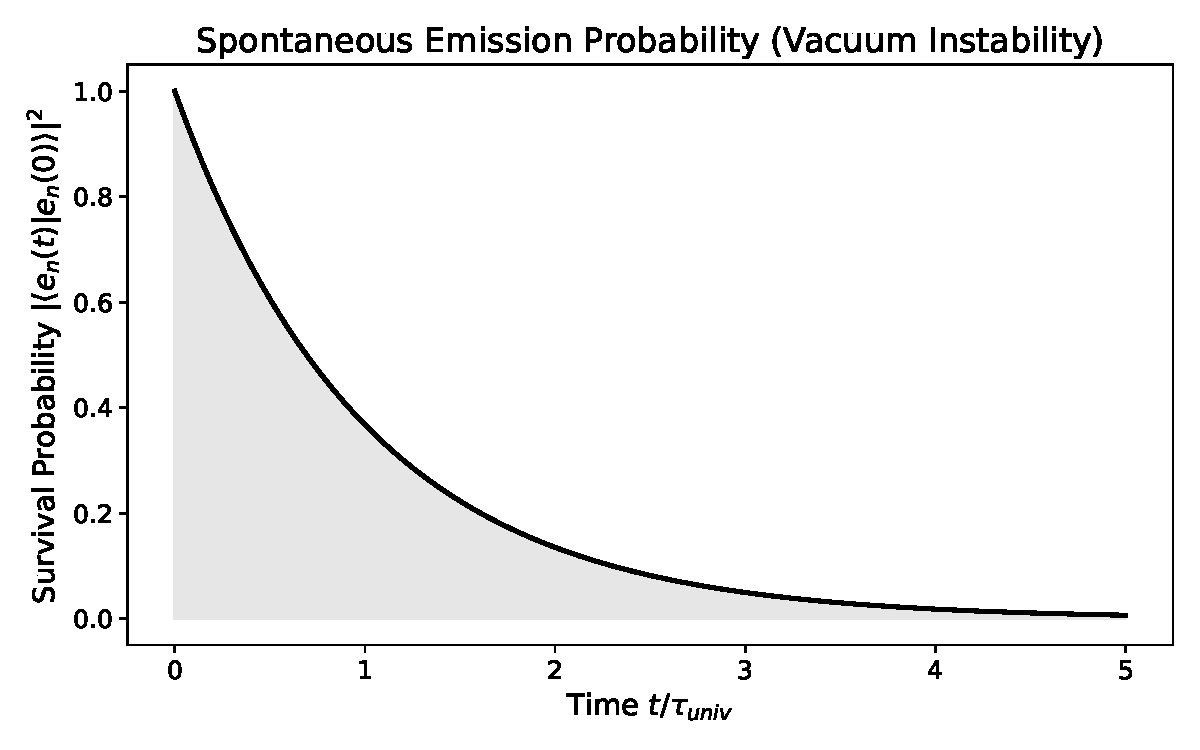
\includegraphics[width=0.85\textwidth]{fig_ch3.pdf}
\caption{Mathematical visualization of the principles derived in Section 3.}
\end{figure}
